\documentclass[a4paper,fleqn]{cas-dc}

\usepackage[spanish,es-tabla,es-nodecimaldot]{babel}
\usepackage[authoryear,round]{natbib}
\bibliographystyle{plainnat}
\newcommand{\autocite}[1]{\citep{#1}}
\newcommand{\parencite}[1]{\citep{#1}}
\usepackage{float}
% cas-dc ya carga graphicx, amsmath, amssymb, booktabs y hyperref
\graphicspath{{figures/}}
\hypersetup{
    linkcolor=blue,
    filecolor=magenta,
    urlcolor=cyan,
    citecolor=blue
}

% Localización de textos fijos de cas-dc
\ExplSyntaxOn
\RenewDocumentCommand \printorcid { } { } % evita la línea "ORCID(s):" vacía
\RenewDocumentEnvironment { keywords } { O{ Palabras~clave } }
   {
     \tex_global:D \tex_setbox:D \g_stm_key_box = \vtop \bgroup
     \hsize=.25 \textwidth
     \cs_set:Npn \sep { \par }
     \parindent = 0pt
     I\,N\,F\,O\,R\,M\,A\,C\,I\,Ó\,N \par \skip_vertical:n { -3pt }
     \rule{.25 \textwidth}{.2pt}\par\footnotesize
     \noindent \textit { #1 }:  \par
   }
   { \egroup }
\ExplSyntaxOff

\begin{document}
\let\WriteBookmarks\relax
\def\floatpagepagefraction{1}
\def\textpagefraction{.001}
\shorttitle{Clasificación automática de 104 tipos de flores}
\shortauthors{Eduardo-Luna et al.}

\title [mode = title]{Clasificación automática de 104 tipos de flores con redes neuronales profundas}
\tnotemark[1]
\tnotetext[1]{Situación problema: Metodología. Diseño de Redes Neuronales y Aprendizaje Profundo (TC2035.201). Basado en la competencia \textit{Petals to the Metal -- Flower Classification on TPU} (Kaggle).}

\author[1]{Angel Eduardo-Luna}
\fnmark[1]
\author[1]{Andrea Estefanía De la Peña Contreras}
\fnmark[2]
\author[1]{Jannette Cristina Flores Rodríguez}
\fnmark[3]
\author[1]{Rey Iván de la Fuente Chávez}
\fnmark[4]
\author[1]{Andrés Huerta Robinson}
\fnmark[5]

\affiliation[1]{organization={Escuela de Ingeniería y Ciencias, Tecnológico de Monterrey},
    city={Monterrey},
    state={Nuevo León},
    country={México}}

\fntext[1]{Matrícula: A00842657}
\fntext[2]{Matrícula: A00840973}
\fntext[3]{Matrícula: A01255711}
\fntext[4]{Matrícula: A01709445}
\fntext[5]{Matrícula: A00838626}

\begin{abstract}
Este trabajo aborda el problema de clasificación automática de imágenes de flores utilizando técnicas de aprendizaje automático y redes neuronales profundas. Se utiliza el conjunto de datos de la competencia \textit{Petals to the Metal -- Flower Classification on TPU} de Kaggle, compuesto por 23,847 imágenes RGB distribuidas entre 104 clases distintas de flores. El conjunto presenta variaciones importantes en tamaño, color, iluminación, orientación y composición de las imágenes, además de un desbalance en la cantidad de ejemplos disponibles para cada clase.

La tarea consiste en desarrollar un modelo capaz de identificar correctamente la clase de una flor a partir de una imagen. Debido a la similitud visual entre algunas categorías y a la variabilidad dentro de una misma clase, se considera principalmente el uso de redes neuronales convolucionales (CNN), ya que permiten extraer automáticamente características relevantes como formas, bordes, colores y patrones visuales. También se consideran arquitecturas previamente desarrolladas, como ResNet, AlexNet e Inception, así como métodos tradicionales de aprendizaje automático, entre ellos KNN, bosques aleatorios y máquinas de vectores de soporte, con el objetivo de comparar distintas alternativas para la solución del problema.

Para evaluar el desempeño se considera especialmente la métrica F1 macro utilizada por Kaggle, ya que asigna la misma importancia a cada una de las 104 clases independientemente de la cantidad de imágenes disponibles. De esta forma, el proyecto busca seleccionar y posteriormente implementar una estrategia de clasificación que logre un buen desempeño general sin favorecer únicamente a las clases con mayor cantidad de ejemplos.
\end{abstract}

\begin{keywords}
Clasificación de imágenes \sep
Redes neuronales convolucionales \sep
Aprendizaje profundo \sep
F1 macro \sep
Kaggle
\end{keywords}


\maketitle

\section{Resumen y objetivos}

Este avance compara una red totalmente conectada de referencia con la CNN
original del equipo y con una segunda CNN que agrega dos capas convolucionales.
Además, evalúa una intervención de regularización sobre la arquitectura original.
El objetivo es medir si extraer patrones espaciales mejora la clasificación de
104 categorías de flores y si aumentar la profundidad o regularizar mejora la
generalización. Se reportan exactitud, F1 macro, pérdida y matrices de confusión
sobre la misma partición de validación.

Para responder a la observación sobre las representaciones de los modelos,
se incorporan diagramas de arquitectura con dimensiones, curvas comparables de
entrenamiento y validación, y ejemplos de aciertos y errores. El notebook adjunto
contiene las llamadas de entrenamiento y las salidas de la evaluación.

La red totalmente conectada se reconstruye para esta comparación a partir del
cargador y del ciclo de entrenamiento existentes. No se encontró en el repositorio
un modelo totalmente conectado identificado como la entrega del Avance 3; por
ello no se atribuyen a aquella entrega los resultados de esta referencia.

\section{Contexto del problema}
Muchas categorías de flores son visualmente parecidas y distinguirlas puede requerir conocimiento especializado. Identificarlas de forma manual es lento cuando se tienen miles de fotografías. Por eso resulta útil contar con modelos que reconozcan la clase de una flor a partir de una imagen.

Este proyecto parte de la competencia "Petals to the Metal", encontrado en Kaggle, cuyo reto es construir un modelo que identifique el tipo de flor en un conjunto de imágenes. La competencia se limita a 104 clases de flores, y consiste en un problema de clasificación multiclase de imágenes en el que el modelo debe tener la capacidad de identificar valores finos como la forma, estructura y color para distinguir entre categorías cercanas. 

Este problema tiene varias dificultades que lo hacen relevante desde un enfoque de redes neuronales. Primeramente, las clases son heterogéneas, ya que algunas de ellas solo tienen un subtipo de flor y otras agrupan muchas subvariedades. Además, las imágenes de las flores no fueron capturadas en el mismo entorno, dando más variedad a las mismas. Por último, el número de imágenes por cada clase tampoco es uniforme, por lo que, considerando la métrica de evaluación, es un punto fuerte a tomar en cuenta que el modelo funcione de manera efectiva tanto para clases con pocos ejemplos como también para aquellas con muchos. 

\section{Descripción del dataset}
\subsection{Origen}
Los datos vienen de \textit{Petals to the Metal -- Flower Classification on TPU}, una competencia \textit{Getting Started} de Kaggle cuyo objetivo es aprender a entrenar modelos en TPU \parencite{kagglePetalsMetal}. Según la descripción de la competencia, las imágenes se tomaron de cinco conjuntos de datos públicos. Algunas clases son muy específicas (por ejemplo, \textit{pink primrose}, que contiene un solo subtipo de flor) y otras agrupan muchas subvariedades (por ejemplo, \textit{wild rose}).

Al revisar la lista de clases nos dimos cuenta de que las primeras 102 siguen exactamente el orden del conjunto Oxford 102 Flowers (Nilsback y Zisserman, 2008): 94 conservan el mismo nombre y las otras 8 se renombraron, se corrigieron o se ampliaron (por ejemplo, \textit{oxeye daisy} pasó a ser \textit{daisy} y \textit{bearded iris} pasó a ser \textit{iris}). Las dos clases extra son \textit{common tulip} y \textit{wild rose}. Las etiquetas están en inglés, así que usamos los nombres originales en cursiva.

\subsection{Tamaño y estructura}
En total hay 23,847 imágenes a color (RGB) de 104 clases, repartidas como muestra la Tabla~\ref{tab:particiones}. Vienen en formato TFRecord, que junta muchas imágenes en pocos archivos binarios para que la TPU las lea rápido. Cada registro tiene tres campos: \texttt{image} (la foto codificada en JPEG), \texttt{id} (un identificador único) y \texttt{class} (la etiqueta, un entero de 0 a 103). Los registros de prueba no traen \texttt{class}, porque esas etiquetas solo las tiene Kaggle para calificar.

\begin{table}[htbp]
\centering
\caption{Particiones del conjunto de datos.}
\label{tab:particiones}
\small
\begin{tabular}{lrrc}
\hline
Partición & Imágenes & \% & ¿Etiquetado? \\
\hline
Entrenamiento & 12,753 & 53.5 & Sí \\
Validación    &  3,712 & 15.6 & Sí \\
Prueba        &  7,382 & 31.0 & No \\
\hline
Total         & 23,847 & 100.0 & \\
\hline
\end{tabular}
\end{table}

Cada partición viene en 4 resoluciones: $192\times192$, $224\times224$, $331\times331$ y $512\times512$ píxeles, con 16 archivos TFRecord por partición, por lo que la base de datos trae 192 archivos TFRecord (4 resoluciones $\times$ 3 particiones $\times$ 16 archivos) más \texttt{sample\_submission.csv}. Tener varias resoluciones nos conviene porque no todas las arquitecturas se diseñaron para el mismo tamaño de entrada: ResNet50, DenseNet201 y EfficientNetB0 hacen uso de $224\times224$, mientras que las EfficientNet más grandes usan resoluciones mayores. Para dimensionar el problema, una sola imágen de $224\times224$ ya tiene 150,528 valores.

En las ejecuciones de este avance se leen los TFRecord de $224\times224$, pero
se redimensionan las imágenes a $112\times112$ antes de entrar a cualquiera de
los modelos. La resolución de origen y la entrada efectiva de entrenamiento
son, por tanto, distintas. Se conservan las particiones y etiquetas originales.

\subsection{Ejemplos de las imágenes}

La tabla~\ref{tab:ejemplos} muestra algunas clases concretas y lo que cada una nos dice sobre el problema. Además, dentro de una misma clase, las fotos cambian mucho de escala, pose e iluminación \citep{nilsback2008} 


La Figura~\ref{fig:ejemplos} muestra fotos reales del conjunto de entrenamiento.

\begin{figure*}[htbp]
\centering
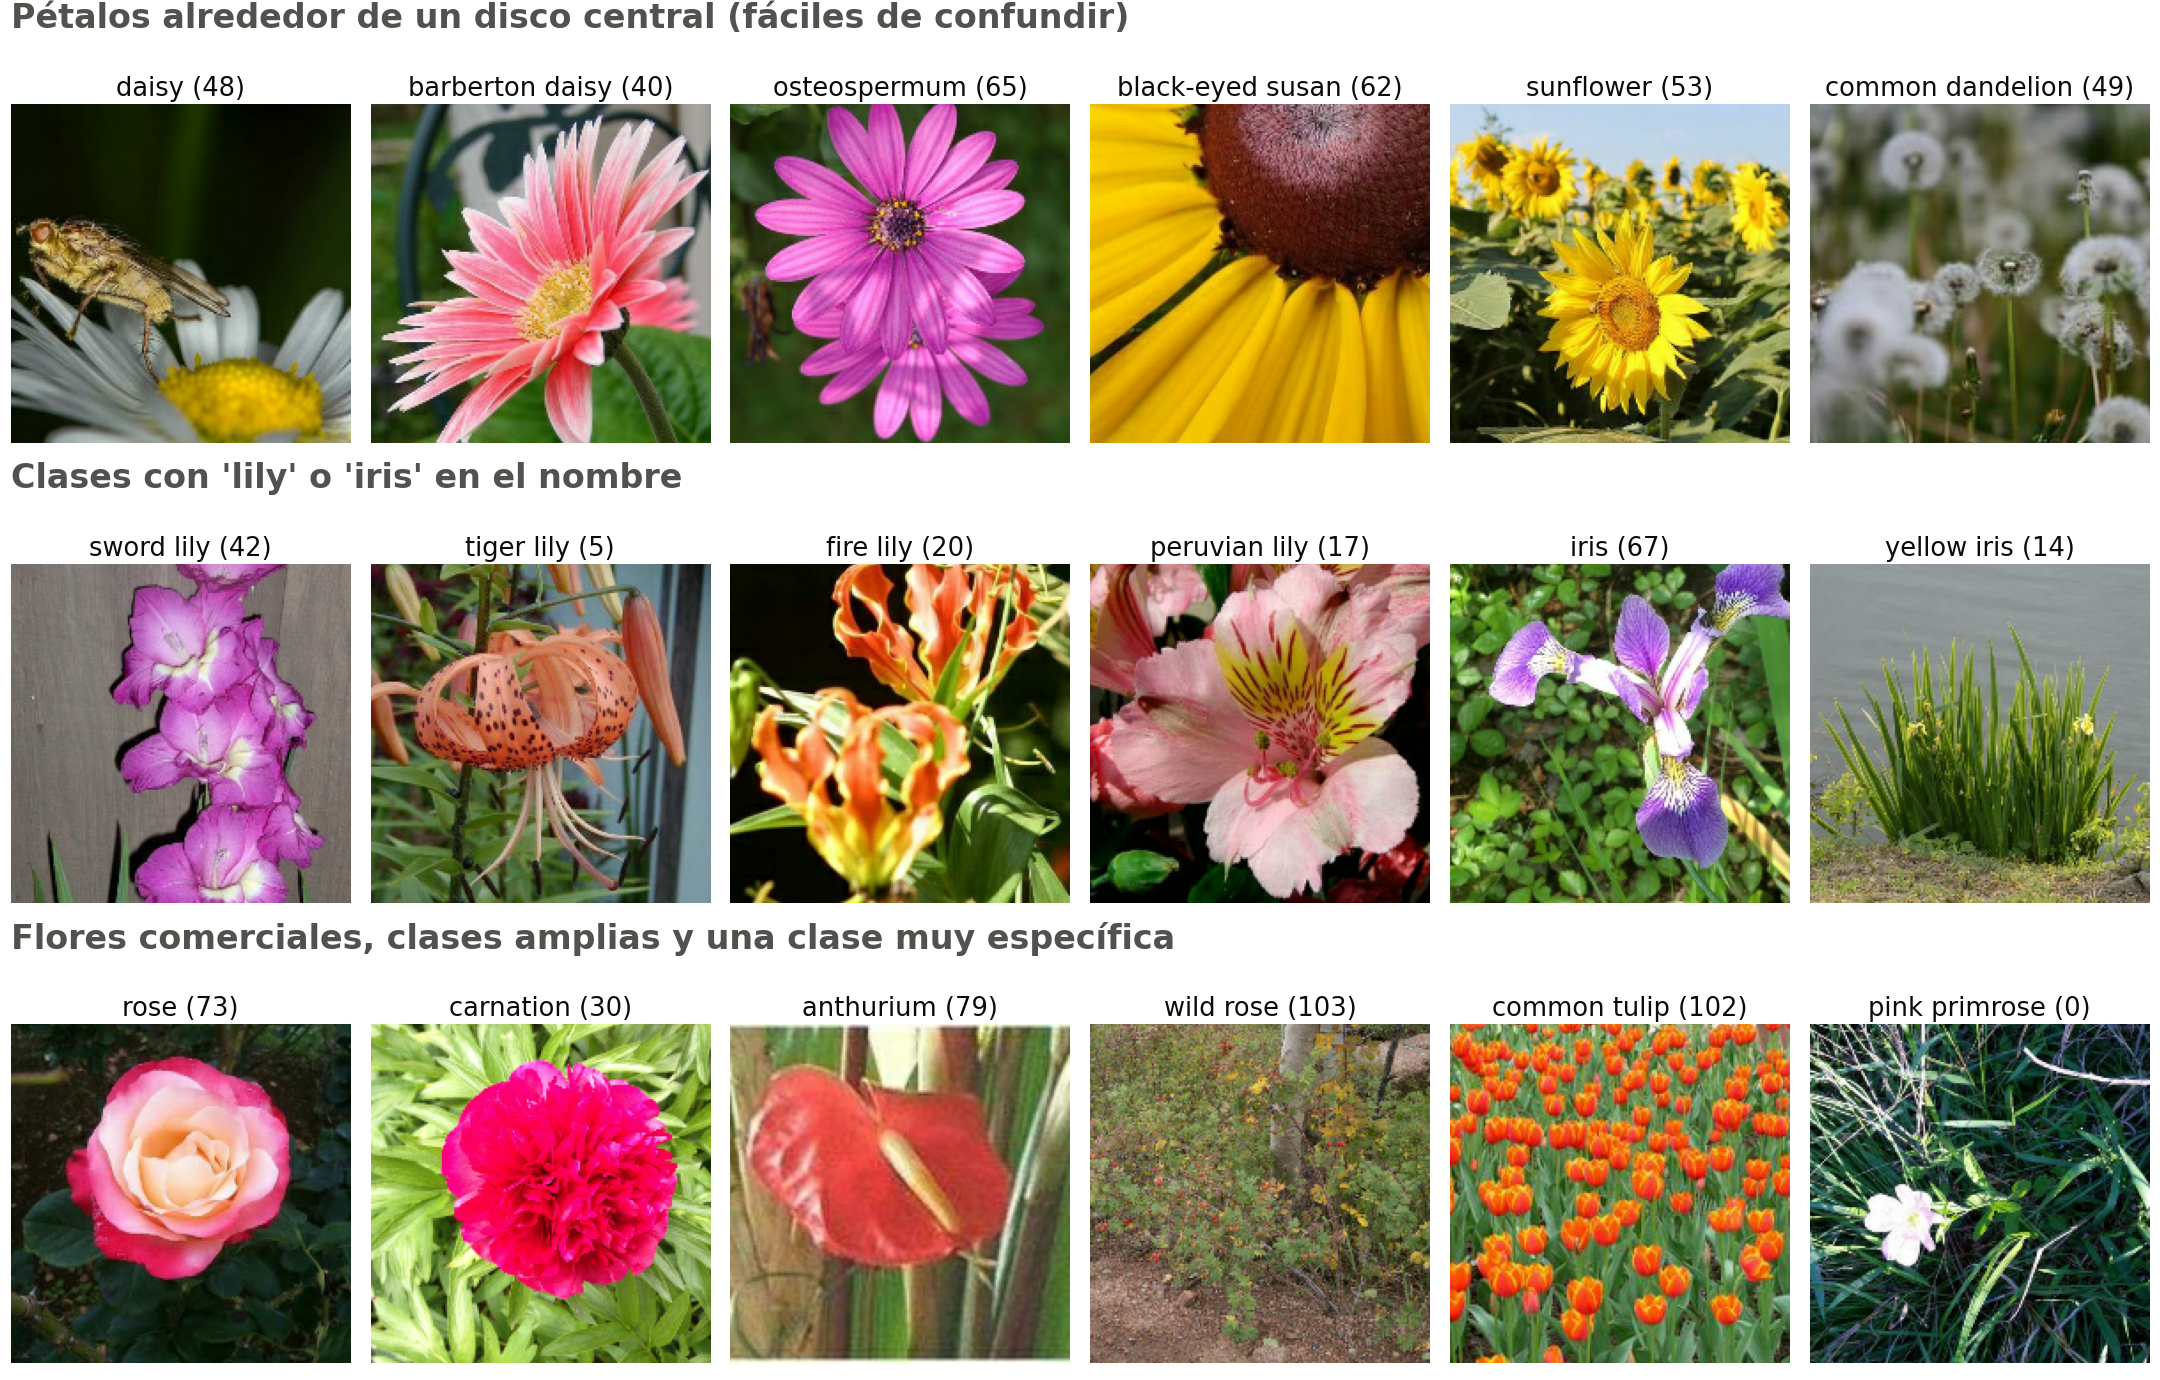
\includegraphics[width=\textwidth]{ejemplos_flores.png}
\caption{Ejemplos reales del conjunto de entrenamiento con su clase y número de etiqueta.}
\label{fig:ejemplos}
\end{figure*}

\begin{table*}[htbp]
\centering
\caption{Clases de ejemplo (nombre y etiqueta) más lo que ilustran.}
\label{tab:ejemplos}
\small
\begin{tabular}{p{0.35\textwidth}p{0.58\textwidth}}
\hline
Clase (etiqueta) & Que ilustra \\
\hline
\textit{sunflower} (53) & Girasol. Flor grande y muy característica. Posiblemente sea de las más fáciles de identificar. \\
\textit{daisy} (48), \textit{barberton daisy} (40), \textit{osteospermum} (65), \textit{black-eyed susan} (62) & Margarita, gerbera, osteospermum y rudbeckia. Todas tienen pétalos alrededor de un disco central. Pueden surgir confusiones entre ellas. \\
\textit{sword lily} (42), \textit{tiger lily} (5), \textit{fire lily} (20), \textit{peruvian lily} (17) & Gladiola, lirio tigre, gloriosa y alstroemeria. Todas dicen \textit{lily}, pero son de cuatro familias botánicas distintas: el modelo tiene que fijarse en la forma, no en el nombre. \\
\textit{iris} (67), \textit{yellow iris} (14) & Misma forma general, la diferencia principal es el color. \\
\textit{rose} (73), \textit{wild rose} (103) & Dos clases de rosas. \textit{Wild rose} es amplia (varias subvariedades) y no viene de Oxford 102. \\
\textit{common tulip} (102) & Tulipán. Clase amplia que tampoco viene de Oxford 102. \\
\textit{pink primrose} (0) & Clase muy específica con un solo subtipo de flor. \\
\textit{carnation} (30) & Clavel, una de las flores comerciales que se producen en el Estado de México. \\
\hline
\end{tabular}
\end{table*}


\subsection{Balance de clases y métrica de evaluación}
Con 12,753 imágenes de entrenamiento y 104 clases, tenemos en promedio 123 imágenes por clase ($12{,}753/104 \approx 122.6$). Sin embargo, las clases no tienen el mismo tamaño: como unas clases agrupan muchas subvariedades y otras solo una, algunas tienen muchas más imágenes que otras.

Por este desbalance, la exactitud no basta: un modelo puede acertar mucho en las clases grandes, fallar en las clases pequeñas y aún verse bien. Por esto mismo, Kaggle califica con el F1 macro \citep{kagglePetalsMetal}. Para cada clase $c$ se calcula la precisión $P_c$, la sensibilidad (\textit{recall}) $R_c$ y su media armónica:

\begin{equation}
P_c=\frac{TP_c}{TP_c+FP_c}, \quad R_c=\frac{TP_c}{TP_c+FN_c},
\end{equation}
\begin{equation}
F1_c=\frac{2\,P_c\,R_c}{P_c+R_c}, \qquad F1_{\text{macro}}=\frac{1}{104}\sum_{c=0}^{103}F1_c,
\end{equation}
donde $TP_c$, $FP_c$ y $FN_c$ son los verdaderos positivos, falsos positivos, y falsos negativos de la clase $c$ . Así todas las clases pesan lo mismo, sin importar cuántas imágenes tengan. 

\subsection{Implicaciones para el proyecto}
Como Kaggle ya separa entrenamiento y validación, no necesitamos hacer nuestra propia partición: entrenaremos con \texttt{train}, elegiremos modelos e hiperparámetros con \texttt{val} y usaremos \texttt{test} solo para la predicción final. Las imagenes vienen en JPEG con valores de 0 a 255, así que habrá que decodificarlas y escalarlas (a $[0,1]$ o con el preprocesamiento que pida cada red preentrenada). Como las etiquetas son enteros,  la red producirá 104 valores de salida, uno por cada clase, que podrán transformarse en probabilidades mediante Softmax. El entrenamiento se
realizará utilizando entropía cruzada categórica dispersa.

\section{Algoritmos y aplicaciones}

Dado el problema planteado, su solucion implica el uso de algoritmos de vision por computadora.

\subsection{Redes Neuronales Convolucionales (CNNs)}

Las redes neuronales convolucionales (CNN) son una alternativa especialmente
adecuada para este problema debido a su capacidad para procesar información
espacial. Mediante filtros convolucionales pueden aprender automáticamente
características de las imágenes, como bordes, texturas y formas. En las capas
internas pueden emplearse funciones de activación como ReLU, mientras que
Softmax puede utilizarse en la salida para representar las probabilidades de
las distintas clases.

\begin{figure}[htbp]
    \centering
    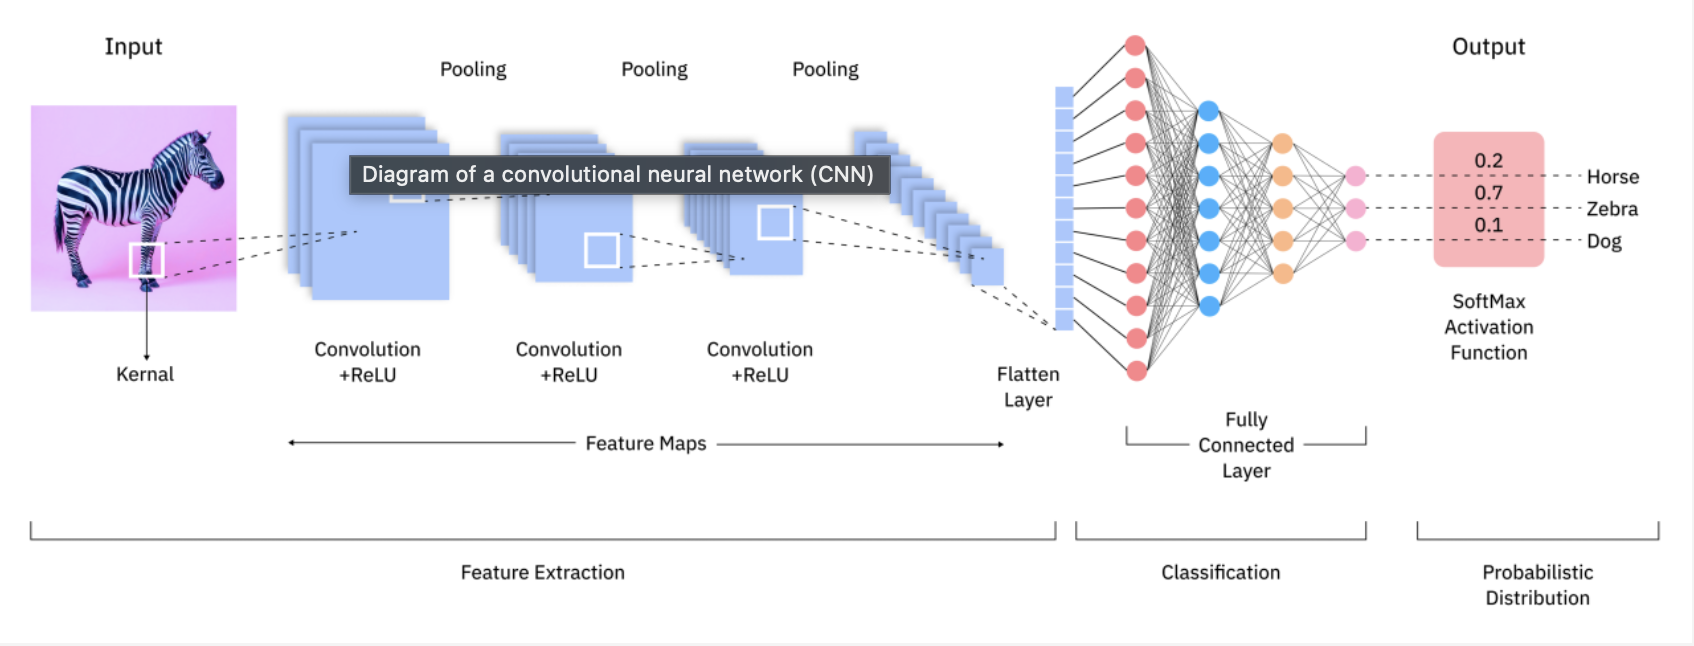
\includegraphics[width=\columnwidth]{cnn_diagram.png}
    \caption{La convolución descompone la imagen en caracteristicas para aprender a clasificar \autocite{ibmWhatImage}.}
    \label{fig:cnn_diagram}
    
\end{figure}


Este método parece ser el principal y el mejor para producir resultados optimos, aunque, dado a la gran cantidad de datos que se tienen que tratar y la variedad de operaciones que se llevan a cabo, hay que considerar que es un metodo lento y computacionalmente pesado. Esto habilita la posibilidad de usar otros algoritmos que se ajusten a la necesidad del problema.

\subsection{Otros algoritmos sin aprendizaje profundo}


\begin{description}
    \item[k vecinos más cercanos (KNN)] Cada imagen lo representa como un vector de características. Usa normalmente la distancia euclidiana para medir las similaridades entre los puntos, y compara con sus k vecinos más cercanos para clasificar la imagen. Es un algoritmo de aprendizaje supervisado.
    \item[Bosque aleatorio] Se compone de un conjunto de árboles de decisión, se calcula la media de los resultados de los árboles.
    \item[Máquinas de Vectores de Soporte (SVMs)] Este algoritmo encuentra la línea óptima para separar dos clases. Una variación llamada SVM multiclase existe para problemas multiclase, como este contexto.
\end{description}


\subsection{Otros modelos de aprendizaje profundo}

\begin{description}
    \item[ResNet] Conocida también como \textit{Residual network}. Útil para entrenar redes neuronales muy profundas. La cota superior para implementar este método es la capacidad de nuestro \textit{hardware} o acceso a equipo computacional que sea capaz de entrenar este tipo de redes más complejas.
    \item[Otros modelos ya implementados] Como \textbf{AlexNet} o \textbf{GoogleNet/inception} que tienen una gran capacidad para reconocer y clasificar imágenes.\autocite{ibmWhatImage}
\end{description}


\subsection{Aplicaciones posibles}

Un modelo capaz de clasificar tipos de flores a partir de imágenes puede tener distintas aplicaciones reales. Una de ellas es la \textbf{identificación automática de plantas}, donde un usuario podría tomar una fotografía y recibir como resultado la especie o clase más probable.


Un ejemplo de este tipo de aplicaciones yace en el apoyo a plataformas de ciencia ciudadana y el monitoreo de biodiversidad. Por ejemplo, iNaturalist ha acumulado más de 300 millones de observaciones hechas por personas comunes \autocite{inaturalist} y utiliza un modelo de visión por computadora, entrenado con esas mismas observaciones, para sugerir la especia a partir de una fotografía. Sin este apoyo automático, cada observación dependería de que una persona la revisara detenidamente, lo que haría el proceso lento y difícil de escalar. Automatizar parte de la tarea ayuda a mejorar la eficiencia y aporta de gran manera a la obtención de datos sobre biodiversidad. Este proyecto es una versión a menor escala de este tipo de sistemas. 

Otra aplicación sería como \textbf{herramienta educativa}, por ejemplo, en aplicaciones para estudiantes o visitantes de jardines botánicos que permitan reconocer flores y consultar información sobre ellas.

Sin embargo, el modelo desarrollado solo podría reconocer las 104 clases presentes en el conjunto de datos, por lo que una aplicación real más amplia requeriría entrenarlo con una mayor variedad de especies.

\section{Metodología}

\subsection{Representación de las arquitecturas implementadas}

La Figura~\ref{fig:arquitecturas-av4} representa los tres diseños entrenados
desde cero. La entrada efectiva es una imagen RGB de $112\times112$ píxeles,
obtenida de los TFRecord de $224\times224$ mediante redimensionamiento bilineal
con antialias. Esto corrige la descripción anterior, que presentaba
$224\times224$ como resolución de entrenamiento.

\begin{figure*}[p]
\centering
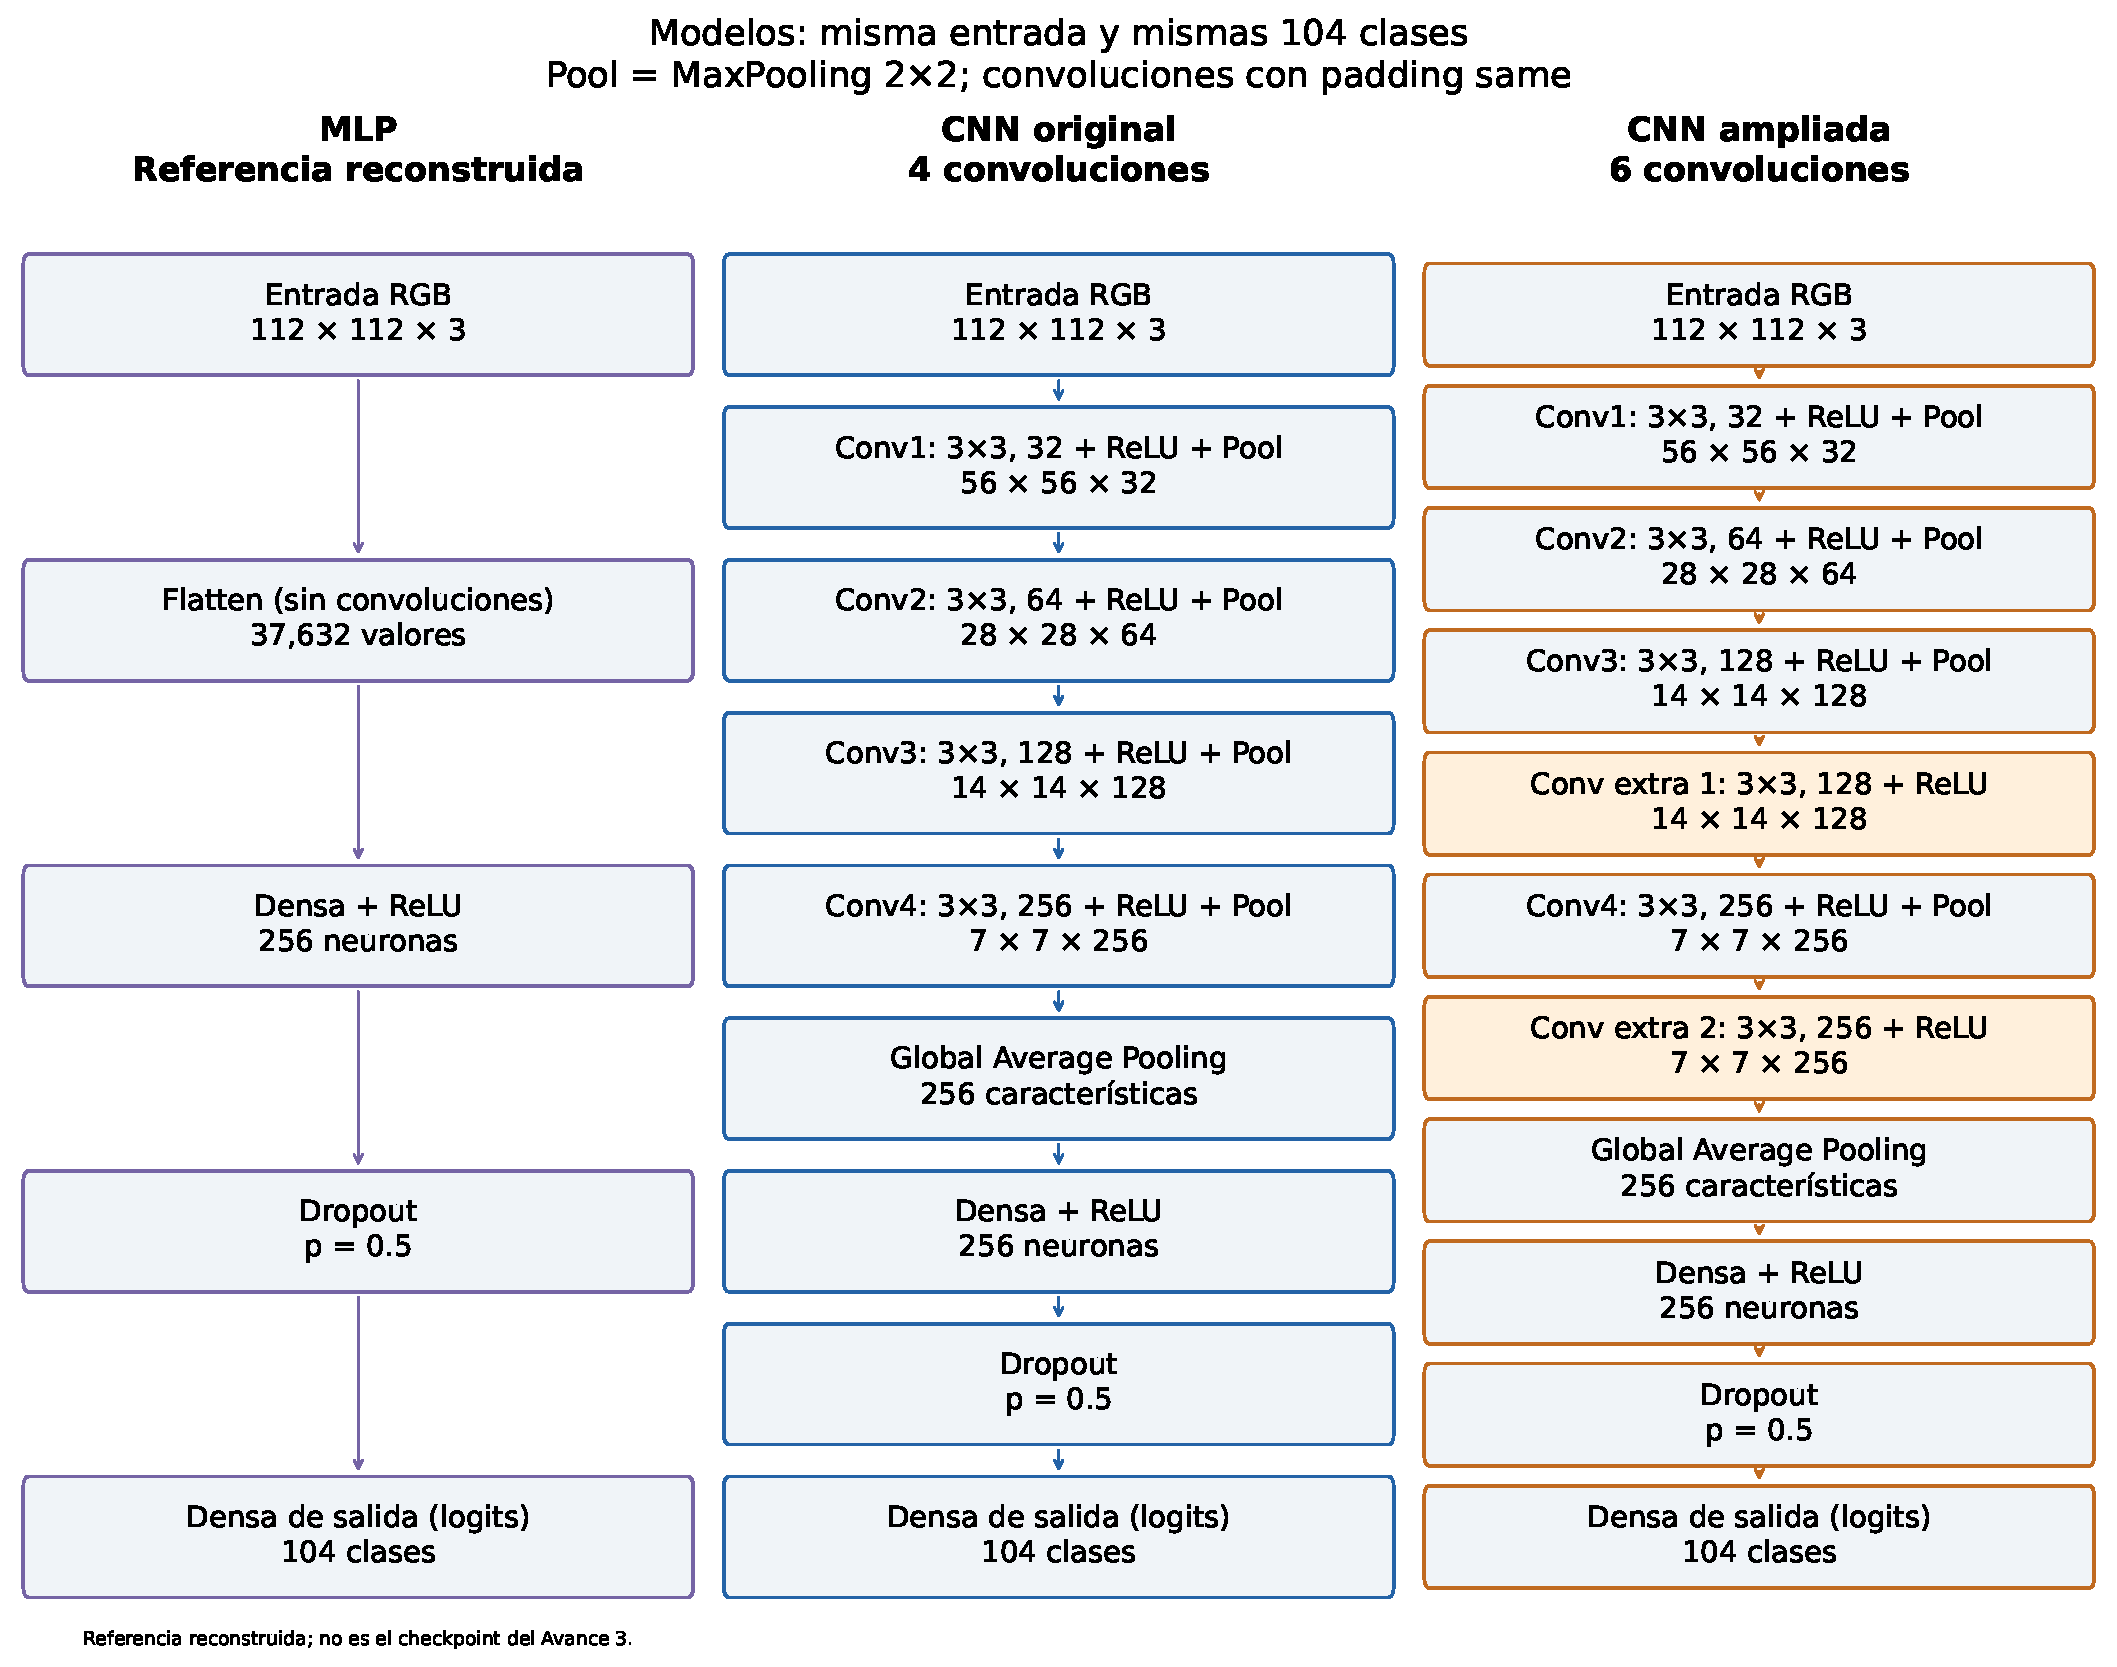
\includegraphics[width=\textwidth,height=0.85\textheight,keepaspectratio]{avance4_2026-10-21/figures/arquitecturas.pdf}
\caption{Representación de la red totalmente conectada de referencia, la CNN
original y la CNN con dos convoluciones adicionales. Las dimensiones corresponden
a las salidas de cada etapa; las capas adicionales se destacan en naranja.
La variante regularizada conserva la arquitectura de la CNN original.}
\label{fig:arquitecturas-av4}
\end{figure*}

La red \textbf{totalmente conectada de referencia} aplana los $112\times112\times3$
valores de entrada en un vector de 37,632 componentes. Aplica una capa densa de
256 unidades con ReLU, dropout de 0.5 y una salida de 104 logits. No contiene
convoluciones ni pooling. Es una comparación reconstruida, como se aclara en la
sección 1, y utiliza el mismo cargador, aumentos y ciclo de entrenamiento que la CNN.

La \textbf{CNN original} emplea cuatro convoluciones de $3\times3$, padding
\textit{same}, ReLU y 32, 64, 128 y 256 filtros. Cada convolución va seguida de
max pooling de $2\times2$. Las salidas de esos bloques son
$56\times56\times32$, $28\times28\times64$, $14\times14\times128$ y
$7\times7\times256$. Después aplica global average pooling (GAP), una capa densa
de 256 unidades con ReLU, dropout de 0.5 y 104 logits de salida.

La \textbf{CNN ampliada} agrega dos capas convolucionales ocultas: una de 128
filtros después del tercer pooling y otra de 256 después del cuarto. Ambas usan
kernel $3\times3$, padding \textit{same} y ReLU, sin pooling adicional. Por tanto,
esta versión tiene seis convoluciones. No se trata de dos capas densas nuevas.

La convolución comparte los pesos del filtro entre posiciones y analiza
vecindarios de píxeles. Así puede aprender bordes, texturas y partes de pétalos
antes de combinarlos. Una capa densa sobre píxeles aplanados asigna pesos
independientes a cada posición y no impone esta estructura local. Esta diferencia
motiva la comparación, pero la mejora debe comprobarse con las métricas.

\subsection{Preprocesamiento y aumento de datos}

Se decodifica cada JPEG como RGB, se convierten sus valores a float32, se
normalizan mediante $x_{\mathrm{norm}}=x/255$ y se redimensionan a $112\times112$.
Las etiquetas son enteros entre 0 y 103. Se mantiene la separación de archivos
original entre entrenamiento y validación, sin incorporar imágenes de validación
al entrenamiento.

Solo en entrenamiento se aplican volteo horizontal, rotación aleatoria de factor
0.05, zoom de 0.1 y contraste de 0.1. Los valores resultantes se recortan a $[0,1]$.
Los aumentos se calculan después de la caché y del mezclado, por lo que cambian
entre épocas. La validación usa imágenes deterministas sin aumentos.

\subsection{Pérdida y actualización de parámetros}

Los modelos producen 104 logits $z_k$. La entropía cruzada se calcula directamente
sobre ellos, sin añadir una segunda softmax a la pérdida:
\begin{equation}
L=-\log\left(\frac{\exp(z_c)}{\sum_{k=1}^{104}\exp(z_k)}\right),
\end{equation}
donde $c$ es la clase verdadera. Para visualizar la confianza se transforma la
salida mediante softmax; esta confianza no constituye una evaluación de calibración.

La referencia totalmente conectada y ambas CNN sin la intervención adicional
usan Adam con tasa inicial $10^{-3}$ y lotes de 64 imágenes. La variante
regularizada usa AdamW y un ajuste de tasa que se detalla en la sección 7.
Se entrena con PyTorch/DirectML en la GPU AMD Radeon RX 6700S, conservando el
cargador y los aumentos de TensorFlow. El mejor checkpoint se exporta a Keras
y se comprueba que mantiene los logits y las predicciones sobre un lote de control.

\subsection{Imágenes sintéticas: experimento independiente}

El proyecto también incluye destilación de datos mediante Distribution Matching
(DM). IPC 1 significa una imagen sintética por cada una de las 104 clases, es
decir, 104 imágenes; IPC 10 significa 1,040. El generador utiliza el extractor
convolucional de la arquitectura original con pesos aleatorios que se renuevan
durante la optimización de los píxeles. No utiliza como generador el checkpoint
entrenado de aproximadamente 63\% de exactitud. Estas figuras históricas se
conservan separadas; los experimentos principales de este avance entrenan con
las 12,753 imágenes reales y no se atribuyen sus métricas a los conjuntos sintéticos.


\section{Protocolo experimental y correcciones}

\subsection{Condiciones de comparación}

Se usan los mismos 12,753 ejemplos reales de entrenamiento y 3,712 de validación,
104 clases, entrada $112\times112$, lote de 64 y semilla 0. Se permiten hasta 150
épocas. Se guarda el checkpoint con el mayor F1 macro de validación; por ello,
la exactitud final reportada corresponde a ese mismo checkpoint y no al máximo
independiente de exactitud. La referencia totalmente conectada y las dos CNN
comparadas por profundidad comparten optimizador, aumentos, dropout y paciencia
de cinco evaluaciones sin mejora. La intervención combinada de regularización
permite una paciencia mayor y cambia el optimizador y su tasa; no es una ablación
aislada de cada técnica.

Las curvas contienen métricas de entrenamiento con aumentos y dropout activos,
mientras que la validación se calcula sin ellos. Por esta razón, una exactitud
de validación mayor que la de entrenamiento no implica por sí sola fuga de datos.
Para diagnosticar sobreajuste se examinan conjuntamente la tendencia de la
pérdida, la exactitud y F1 macro, sin usar únicamente la distancia entre dos curvas.

La comparación se limita a una semilla y utiliza validación para seleccionar
épocas e hiperparámetros. No proporciona intervalos de confianza ni una medida
final independiente de generalización. El conjunto de prueba de Kaggle carece
de etiquetas locales; no se presentan los resultados de validación como
exactitud de prueba ni como puntaje de la competencia.

La semilla y las configuraciones se guardan para repetir el procedimiento, pero
las operaciones de GPU y la canalización paralela no garantizan resultados
idénticos bit a bit. Las métricas históricas y las nuevas ejecuciones se identifican
por separado en sus respectivas carpetas.

\subsection{Trazabilidad y ajustes del documento}

Las ejecuciones nuevas se guardan bajo \texttt{reports/avance4\_2026-10-21}, con
configuraciones, históricos por época, checkpoints y predicciones por imagen.
Las figuras se exportan tanto a PNG para presentación como a PDF para el reporte.
Un manifiesto registra la versión del código y sus hashes; los experimentos
anteriores se conservan y no se mezclan con las métricas nuevas.

Respecto del documento anterior, las secciones 1 a 6 ahora explicitan los
objetivos medibles, la resolución realmente usada y el lote de 64; representan
las arquitecturas y la ubicación exacta de las dos capas nuevas; distinguen la
referencia totalmente conectada de la CNN original; separan destilación y
clasificación; y aclaran el criterio de selección y el alcance de la validación.
Se atiende la observación compartida sobre las representaciones de los modelos.
No se dispone del texto completo de la retroalimentación del Avance 3, por lo que
no se afirma haber atendido observaciones adicionales no documentadas.




\nocite{*}
\bibliography{references}
\end{document}
